% =====================================================================
%  Proyecto Aprendizaje por Refuerzo - Entrega final
%  Implementación, entrenamiento y evaluación del agente
%  Compilar con pdfLaTeX:  latexmk -pdf reporte_final.tex
%  Las cifras y tablas de generado/ las produce experiments/report_numbers.py
% =====================================================================
\documentclass[11pt,letterpaper]{article}

% ---------- Idioma y codificación ----------
\usepackage[T1]{fontenc}
\usepackage[utf8]{inputenc}
\usepackage{babel}
\babelprovide[import,main]{spanish}
\usepackage{lmodern}

% ---------- Página ----------
\usepackage[margin=2.3cm]{geometry}
\usepackage{fancyhdr}
\usepackage{titlesec}
\usepackage{parskip}

% ---------- Matemáticas, tablas y figuras ----------
\usepackage{amsmath,amssymb}
\usepackage{booktabs}
\usepackage{tabularx}
\usepackage{array}
\usepackage{multirow}
\usepackage[table]{xcolor}
\usepackage{enumitem}
\usepackage{caption}
\usepackage{graphicx}
\usepackage{float}
\usepackage[colorlinks=true,linkcolor=azul,urlcolor=azul]{hyperref}

% ---------- Colores y estilo ----------
\definecolor{azul}{HTML}{1F4E79}
\definecolor{gris}{HTML}{F2F4F7}
\titleformat{\section}{\Large\bfseries\color{azul}}{\thesection.}{0.6em}{}
\titleformat{\subsection}{\large\bfseries\color{azul}}{\thesubsection}{0.6em}{}
\captionsetup{font=small,labelfont=bf}
\setlist{itemsep=2pt,topsep=4pt}
\newcolumntype{L}{>{\raggedright\arraybackslash}X}
\newcolumntype{R}{>{\raggedleft\arraybackslash}X}
\newcolumntype{P}[1]{>{\raggedright\arraybackslash}p{#1}}
\renewcommand{\arraystretch}{1.25}
\graphicspath{{../../results/figures/}{../../results/entrega1/figures/}}

\pagestyle{fancy}
\fancyhf{}
\lhead{\small Aprendizaje por Refuerzo -- Proyecto, entrega final}
\rhead{\small Consolidación de picking en un CD}
\cfoot{\small \thepage}

% ---------- Macros ----------
\newcommand{\LOTE}[1]{\mathsf{LOTE}_{#1}}
\newcommand{\URG}{\mathsf{URGENTE}}
\newcommand{\ESP}{\mathsf{ESPERAR}}
\newcommand{\sfin}{s_{\mathrm{fin}}}
\newcommand{\umax}{u_{\max}}
% Rutas en monoespaciada que pueden partirse después de / y _
\newcommand{\code}[1]{{\ttfamily\codebreaks#1\endcodebreaks}}
\makeatletter
\def\codebreaks#1\endcodebreaks{\@codebreaks#1\@nil}
\def\@codebreaks#1{\ifx#1\@nil\else\ifx#1/\slash\else\ifx#1\_\_\allowbreak\else#1\fi\fi\expandafter\@codebreaks\fi}
\makeatother
\setlength{\emergencystretch}{2em}
\makeatletter\newcommand{\filas}[1]{\@@input #1 }\makeatother  % \input primitivo: funciona dentro de tablas

\newcommand{\QLR}{$-$599}
\newcommand{\QLRci}{339}
\newcommand{\QLV}{33{,}9}
\newcommand{\QLVci}{7{,}9}
\newcommand{\QLP}{6{,}7}
\newcommand{\QLT}{89{,}2}
\newcommand{\QLVL}{0{,}584}
\newcommand{\QLW}{62{,}3}
\newcommand{\QLViajes}{80{,}6}
\newcommand{\QLLlegadas}{356{,}9}
\newcommand{\QLCkpt}{6\,000}
\newcommand{\QLEstados}{3\,335}
\newcommand{\EQLR}{$-$1\,296}
\newcommand{\EQLRci}{413}
\newcommand{\EQLV}{78{,}6}
\newcommand{\EQLVci}{11{,}7}
\newcommand{\EQLP}{27{,}2}
\newcommand{\EQLT}{74{,}5}
\newcommand{\EQLVL}{0{,}583}
\newcommand{\EQLW}{87{,}7}
\newcommand{\EQLViajes}{77{,}9}
\newcommand{\EQLLlegadas}{356{,}9}
\newcommand{\EQLCkpt}{3\,500}
\newcommand{\EQLEstados}{1\,778}
\newcommand{\SARSAR}{$-$732}
\newcommand{\SARSARci}{331}
\newcommand{\SARSAV}{33{,}5}
\newcommand{\SARSAVci}{7{,}8}
\newcommand{\SARSAP}{7{,}9}
\newcommand{\SARSAT}{88{,}9}
\newcommand{\SARSAVL}{0{,}583}
\newcommand{\SARSAW}{64{,}5}
\newcommand{\SARSAViajes}{77{,}1}
\newcommand{\SARSALlegadas}{356{,}9}
\newcommand{\SARSACkpt}{1\,000}
\newcommand{\SARSAEstados}{2\,178}
\newcommand{\ESARSAR}{$-$858}
\newcommand{\ESARSARci}{319}
\newcommand{\ESARSAV}{72{,}3}
\newcommand{\ESARSAVci}{10{,}2}
\newcommand{\ESARSAP}{19{,}8}
\newcommand{\ESARSAT}{76{,}9}
\newcommand{\ESARSAVL}{0{,}576}
\newcommand{\ESARSAW}{80{,}1}
\newcommand{\ESARSAViajes}{74{,}6}
\newcommand{\ESARSALlegadas}{356{,}9}
\newcommand{\ESARSACkpt}{5\,000}
\newcommand{\ESARSAEstados}{2\,053}
\newcommand{\MCR}{$-$2\,433}
\newcommand{\MCRci}{688}
\newcommand{\MCV}{70{,}7}
\newcommand{\MCVci}{14{,}6}
\newcommand{\MCP}{18{,}3}
\newcommand{\MCT}{77{,}7}
\newcommand{\MCVL}{0{,}590}
\newcommand{\MCW}{76{,}8}
\newcommand{\MCViajes}{87{,}5}
\newcommand{\MCLlegadas}{356{,}9}
\newcommand{\MCCkpt}{6\,000}
\newcommand{\MCEstados}{2\,997}
\newcommand{\EMCR}{$-$3\,792}
\newcommand{\EMCRci}{566}
\newcommand{\EMCV}{160{,}7}
\newcommand{\EMCVci}{14{,}9}
\newcommand{\EMCP}{58{,}5}
\newcommand{\EMCT}{51{,}3}
\newcommand{\EMCVL}{0{,}607}
\newcommand{\EMCW}{124{,}0}
\newcommand{\EMCViajes}{105{,}2}
\newcommand{\EMCLlegadas}{356{,}9}
\newcommand{\EMCCkpt}{2\,000}
\newcommand{\EMCEstados}{1\,514}
\newcommand{\UrgR}{$-$426}
\newcommand{\UrgRci}{307}
\newcommand{\UrgV}{33{,}8}
\newcommand{\UrgVci}{7{,}2}
\newcommand{\UrgP}{5{,}6}
\newcommand{\UrgT}{89{,}3}
\newcommand{\UrgVL}{0{,}592}
\newcommand{\UrgW}{58{,}1}
\newcommand{\UrgViajes}{90{,}7}
\newcommand{\UrgLlegadas}{356{,}9}
\newcommand{\EUrgR}{873}
\newcommand{\EUrgRci}{205}
\newcommand{\EUrgV}{33{,}3}
\newcommand{\EUrgVci}{7{,}2}
\newcommand{\EUrgP}{5{,}6}
\newcommand{\EUrgT}{89{,}5}
\newcommand{\EUrgVL}{0{,}590}
\newcommand{\EUrgW}{58{,}6}
\newcommand{\EUrgViajes}{88{,}1}
\newcommand{\EUrgLlegadas}{356{,}9}
\newcommand{\UmbralR}{$-$561}
\newcommand{\UmbralRci}{308}
\newcommand{\UmbralV}{34{,}8}
\newcommand{\UmbralVci}{7{,}4}
\newcommand{\UmbralP}{5{,}9}
\newcommand{\UmbralT}{88{,}9}
\newcommand{\UmbralVL}{0{,}585}
\newcommand{\UmbralW}{59{,}8}
\newcommand{\UmbralViajes}{75{,}1}
\newcommand{\UmbralLlegadas}{356{,}9}
\newcommand{\EUmbralR}{693}
\newcommand{\EUmbralRci}{204}
\newcommand{\EUmbralV}{35{,}7}
\newcommand{\EUmbralVci}{7{,}5}
\newcommand{\EUmbralP}{6{,}5}
\newcommand{\EUmbralT}{88{,}5}
\newcommand{\EUmbralVL}{0{,}584}
\newcommand{\EUmbralW}{60{,}8}
\newcommand{\EUmbralViajes}{74{,}3}
\newcommand{\EUmbralLlegadas}{356{,}9}
\newcommand{\ConsR}{$-$1\,390}
\newcommand{\ConsRci}{450}
\newcommand{\ConsV}{69{,}6}
\newcommand{\ConsVci}{12{,}6}
\newcommand{\ConsP}{6{,}2}
\newcommand{\ConsT}{79{,}3}
\newcommand{\ConsVL}{0{,}592}
\newcommand{\ConsW}{57{,}9}
\newcommand{\ConsViajes}{90{,}7}
\newcommand{\ConsLlegadas}{356{,}9}
\newcommand{\EConsR}{$-$72}
\newcommand{\EConsRci}{346}
\newcommand{\EConsV}{70{,}7}
\newcommand{\EConsVci}{13{,}0}
\newcommand{\EConsP}{6{,}5}
\newcommand{\EConsT}{79{,}0}
\newcommand{\EConsVL}{0{,}591}
\newcommand{\EConsW}{58{,}6}
\newcommand{\EConsViajes}{88{,}2}
\newcommand{\EConsLlegadas}{356{,}9}
\newcommand{\RandR}{$-$7\,322}
\newcommand{\RandRci}{586}
\newcommand{\RandV}{176{,}1}
\newcommand{\RandVci}{12{,}6}
\newcommand{\RandP}{50{,}5}
\newcommand{\RandT}{46{,}1}
\newcommand{\RandVL}{0{,}607}
\newcommand{\RandW}{124{,}8}
\newcommand{\RandViajes}{102{,}6}
\newcommand{\RandLlegadas}{356{,}9}
\newcommand{\ERandR}{$-$4\,168}
\newcommand{\ERandRci}{413}
\newcommand{\ERandV}{175{,}6}
\newcommand{\ERandVci}{13{,}0}
\newcommand{\ERandP}{50{,}5}
\newcommand{\ERandT}{46{,}3}
\newcommand{\ERandVL}{0{,}605}
\newcommand{\ERandW}{124{,}5}
\newcommand{\ERandViajes}{101{,}0}
\newcommand{\ERandLlegadas}{356{,}9}
\newcommand{\UrgSiempreR}{$-$20\,366}
\newcommand{\UrgSiempreRci}{399}
\newcommand{\UrgSiempreV}{286{,}5}
\newcommand{\UrgSiempreVci}{4{,}3}
\newcommand{\UrgSiempreP}{184{,}1}
\newcommand{\UrgSiempreT}{14{,}7}
\newcommand{\UrgSiempreVL}{0{,}925}
\newcommand{\UrgSiempreW}{360{,}7}
\newcommand{\UrgSiempreViajes}{175{,}8}
\newcommand{\UrgSiempreLlegadas}{356{,}9}
\newcommand{\EUrgSiempreR}{$-$10\,681}
\newcommand{\EUrgSiempreRci}{202}
\newcommand{\EUrgSiempreV}{287{,}3}
\newcommand{\EUrgSiempreVci}{4{,}3}
\newcommand{\EUrgSiempreP}{184{,}6}
\newcommand{\EUrgSiempreT}{14{,}5}
\newcommand{\EUrgSiempreVL}{0{,}925}
\newcommand{\EUrgSiempreW}{362{,}8}
\newcommand{\EUrgSiempreViajes}{175{,}2}
\newcommand{\EUrgSiempreLlegadas}{356{,}9}
\newcommand{\EsperarR}{$-$36\,071}
\newcommand{\EsperarRci}{405}
\newcommand{\EsperarV}{338{,}9}
\newcommand{\EsperarVci}{3{,}9}
\newcommand{\EsperarP}{356{,}9}
\newcommand{\EsperarT}{0{,}0}
\newcommand{\EsperarVL}{0{,}000}
\newcommand{\EsperarW}{660{,}6}
\newcommand{\EsperarViajes}{0{,}0}
\newcommand{\EsperarLlegadas}{356{,}9}
\newcommand{\EEsperarR}{$-$20\,663}
\newcommand{\EEsperarRci}{196}
\newcommand{\EEsperarV}{338{,}9}
\newcommand{\EEsperarVci}{3{,}9}
\newcommand{\EEsperarP}{356{,}9}
\newcommand{\EEsperarT}{0{,}0}
\newcommand{\EEsperarVL}{0{,}000}
\newcommand{\EEsperarW}{660{,}6}
\newcommand{\EEsperarViajes}{0{,}0}
\newcommand{\EEsperarLlegadas}{356{,}9}
\newcommand{\DifQLR}{$-$173}
\newcommand{\DifQLRci}{109}
\newcommand{\DifQLV}{0{,}1}
\newcommand{\DifQLVci}{3{,}6}
\newcommand{\DifQLViajes}{$-$10{,}0}
\newcommand{\DifQLViajesci}{1{,}0}
\newcommand{\DifQLP}{1{,}1}
\newcommand{\DifQLPci}{1{,}0}
\newcommand{\DifQLW}{4{,}3}
\newcommand{\DifQLWci}{0{,}8}
\newcommand{\DifSARSAR}{$-$306}
\newcommand{\DifSARSARci}{109}
\newcommand{\DifSARSAV}{$-$0{,}3}
\newcommand{\DifSARSAVci}{3{,}4}
\newcommand{\DifSARSAViajes}{$-$13{,}5}
\newcommand{\DifSARSAViajesci}{1{,}1}
\newcommand{\DifSARSAP}{2{,}3}
\newcommand{\DifSARSAPci}{0{,}9}
\newcommand{\DifSARSAW}{6{,}4}
\newcommand{\DifSARSAWci}{0{,}8}
\newcommand{\DifEQLR}{$-$2\,169}
\newcommand{\DifEQLRci}{312}
\newcommand{\DifEQLV}{45{,}3}
\newcommand{\DifEQLVci}{8{,}2}
\newcommand{\DifEQLViajes}{$-$10{,}2}
\newcommand{\DifEQLViajesci}{1{,}3}
\newcommand{\DifEQLP}{21{,}6}
\newcommand{\DifEQLPci}{3{,}6}
\newcommand{\DifEQLW}{29{,}1}
\newcommand{\DifEQLWci}{2{,}8}
\newcommand{\DifESARSAR}{$-$1\,731}
\newcommand{\DifESARSARci}{200}
\newcommand{\DifESARSAV}{39{,}0}
\newcommand{\DifESARSAVci}{6{,}2}
\newcommand{\DifESARSAViajes}{$-$13{,}6}
\newcommand{\DifESARSAViajesci}{1{,}3}
\newcommand{\DifESARSAP}{14{,}2}
\newcommand{\DifESARSAPci}{2{,}5}
\newcommand{\DifESARSAW}{21{,}5}
\newcommand{\DifESARSAWci}{1{,}5}
\newcommand{\MejorRegla}{Lote más urgente}
\newcommand{\Episodios}{6\,000}
\newcommand{\TurnosPrueba}{100}
\newcommand{\TurnosValidacion}{20}
\newcommand{\Alpha}{0{,}05}
\newcommand{\GammaF}{0{,}95}
\newcommand{\EpsIni}{0{,}50}
\newcommand{\EpsMin}{0{,}02}
\newcommand{\EGamma}{0{,}99}
\newcommand{\PolSlotecritica}{90}
\newcommand{\PolSloteotra}{2}
\newcommand{\PolSloteconsolidada}{0}
\newcommand{\PolSlote}{0}
\newcommand{\PolSurgente}{2}
\newcommand{\PolSesperar}{6}
\newcommand{\PolDcuatroEsperar}{8}
\newcommand{\PolTurnos}{30}
\newcommand{\PolRestoEsperar}{48}
\newcommand{\PolESlotecritica}{48}
\newcommand{\PolESloteotra}{3}
\newcommand{\PolESloteconsolidada}{0}
\newcommand{\PolESlote}{0}
\newcommand{\PolESurgente}{7}
\newcommand{\PolESesperar}{43}


% =====================================================================
\begin{document}

\begin{center}
  {\small Universidad de los Andes \textperiodcentered{} Maestría en Inteligencia Artificial}\\[2pt]
  {\small Aprendizaje por Refuerzo \textperiodcentered{} Prof. Nicolás Cardozo}\\[10pt]
  {\LARGE\bfseries\color{azul} Agente de RL para la consolidación de órdenes\\[2pt] de picking en un centro de distribución}\\[8pt]
  {\large Entrega final: implementación, entrenamiento y evaluación}\\[8pt]
  Miguel Ángel Muñoz Layton \quad\textperiodcentered\quad Daniel F. Barrera Armendaris\\[2pt]
  {\small Noviembre de 2026}
\end{center}

\vspace{4pt}
\hrule
\vspace{8pt}

\section*{Resumen}

Se implementó el MDP definido en la Entrega 1 como un simulador compatible con Gymnasium y se
entrenaron tres agentes tabulares (Q-learning, SARSA y Monte Carlo) durante \Episodios{} turnos de
8 horas. El agente entregado, Q-learning, reduce las órdenes vencidas de \RandV{} por turno (agente sin
entrenar, que actúa al azar) a \QLV{}, y mejora la recompensa media de \RandR{} a \QLR{}. Así alcanza el nivel de servicio
de la mejor regla fija diseñada a mano (\MejorRegla{}, \UrgV{} órdenes vencidas) con \DifQLViajes{}
viajes por turno: aprendió a esperar para consolidar cuando no hay urgencia. A cambio mantiene más
WIP y en recompensa total queda por debajo de esa regla.

Los estados y las acciones son exactamente los entregados. La función de recompensa y la regla de avance
del reloj se ajustaron, y la sección~\ref{sec:cambios} justifica cada cambio. La evidencia es directa: con
la especificación entregada, el mismo algoritmo vence \EQLV{} órdenes por turno, mientras que la misma
regla fija vence \EUrgV{}. Con esa recompensa, el agente aprendía a esperar con órdenes críticas pendientes.



% =====================================================================
\section{El problema y el ambiente}

Un centro de distribución recibe órdenes durante un turno de 8 horas. Cada orden tiene entre 1 y 6
líneas (un SKU cada una) repartidas en zonas de racks y un deadline. Un agente decide, cada vez que hay
operarios libres, qué trabajo liberar: un lote consolidado de una zona, la orden más urgente completa
o esperar. Consolidar ahorra visitas, porque varias órdenes que piden el mismo SKU se recogen en una sola
ubicación; esperar permite formar lotes más grandes, pero arriesga los deadlines. La definición formal
del MDP está en la Entrega 1; aquí se resume lo necesario para leer los resultados.

\textbf{Estados.} $s=(w_z, c_z, u_z)_{z\in Z}\cup(o,\lambda)$: por zona, el WIP $w_z\in\{0,\dots,3\}$, la
consolidación $c_z\in\{0,1,2\}$ (cuántas órdenes comparten el SKU más pedido) y la urgencia
$u_z\in\{0,\dots,3\}$ (holgura mínima); además, los operarios libres $o\in\{0,\dots,3\}$ y la demanda
reciente $\lambda\in\{0,1,2\}$. Se usa la versión tabular de 2 zonas que propone la sección 2 de la
Entrega 1, con $28^2\cdot 12+1=9\,409$ estados.

\textbf{Acciones.} $A=\{\LOTE{A},\LOTE{B},\URG,\ESP\}$, con la máscara de la Entrega 1: $\LOTE{z}$ solo si
$o\ge1$ y $w_z\ge1$; $\URG$ si $o\ge1$ y hay trabajo; $\ESP$ siempre, salvo en $\sfin$.

\textbf{Simulador.} El código (\code{src/rl\_warehouse/env/warehouse.py}) es un simulador por eventos
compatible con Gymnasium. Los supuestos que la Entrega 1 no fijaba se resumen en el cuadro~\ref{tab:supuestos}.

\begin{table}[H]
\centering\small
\begin{tabularx}{\textwidth}{@{}P{3.6cm}L@{}}
\toprule
\textbf{Elemento} & \textbf{Supuesto} \\
\midrule
Demanda & Poisson no homogéneo con dos picos: 0,3 órdenes/min en valle y 1,2 en pico (min 60--180 y 270--390). Sin llegadas en los últimos 30 min \\
Órdenes & 1 a 6 líneas, zona uniforme, deadline entre 30 y 120 min desde la llegada \\
SKU & 30 por zona con popularidad Zipf ($s=1$), como una curva ABC: pocos SKU concentran la demanda \\
Tiempo de recogida & 4 min de desplazamiento $+$ 1 min por ubicación visitada $+$ 0,2 min por línea \\
Operarios y carro & 3 operarios; hasta 20 líneas por lote \\
\bottomrule
\end{tabularx}
\caption{Supuestos del simulador (\code{configs/env\_default.yaml}).}
\label{tab:supuestos}
\end{table}

Con estos supuestos el problema tiene tensión real: en los picos llegan más órdenes de las que tres
operarios recogen sin consolidar, así que la política importa. En una primera versión con demanda
constante de 0,5 órdenes/min ninguna orden vencía, ni siquiera con una política aleatoria, y por tanto no
había nada que aprender.

% =====================================================================
\section{De la especificación entregada a la especificación final}
\label{sec:cambios}

Los estados, su discretización y las acciones se implementaron exactamente como se entregaron. La
función de recompensa y la regla de avance del reloj sí se ajustaron después de entrenar los primeros
agentes. Las dos versiones están implementadas y se pueden ejecutar
(\code{configs/env\_entrega1.yaml} y \code{configs/env\_default.yaml}); las pruebas automáticas
\code{test\_entrega1\_*} reproducen, con el esquema entregado, las triplas $(s,a,s')$ del cuadro 9 de la
Entrega 1 (T1, T3, T4, T6, T8 y T9) y el texto que lo acompaña.

\begin{table}[H]
\centering\footnotesize
\begin{tabularx}{\textwidth}{@{}P{2.3cm}P{3.6cm}P{3.6cm}L@{}}
\toprule
\textbf{Elemento} & \textbf{Entrega 1} & \textbf{Final} & \textbf{Motivo} \\
\midrule
Pago de $\LOTE{z}$ & $P_c(c_z)+B_u(u_z)$: de $+1$ a $+18$ por lote & $+2$ por visita ahorrada ($\ell-v$) y $-1$ por viaje & El bono se cobra por lote: partir el trabajo en muchos lotes pequeños paga más que uno grande. Además $c_z$ mide el SKU más compartido de la zona, no lo que el lote ahorra de verdad \\
$\URG$ & $+8$, $+1$ o $-4$ según $\umax$ & $-1$ por viaje; $-5$ si $\umax=1$ & El $+8$ premiaba la urgencia dos veces (ya la castiga el $-20$ por vencimiento) y pagaba casi lo mismo que un lote de la zona crítica ($+9$ a $+18$), aunque una orden suelta no consolida \\
$\ESP$ con $\lambda=2$ y $c\le1$ & $+2$ & $0$ & Un pago positivo por esperar en un estado que se repite puede crear un ciclo de recompensa: esperar paga por sí mismo y no por el lote que se forma. Con el costo de WIP, el beneficio de esperar llega por las visitas que ahorra el lote siguiente \\
Congestión & $-2$ por zona con $w'_z=3$ & $-0{,}05$ por línea sin asignar por minuto & La saturación binaria no distingue 16 de 60 líneas ni cuánto tiempo esperan. El costo de WIP es proporcional y hace que esperar nunca sea gratis \\
Urgencia & Solo $-20$ al vencer & $-1$ por zona crítica en $s'$ & Señal densa: el agente recibe la consecuencia antes del vencimiento \\
Descuido & $-6$ & $-10$ & Ignorar una orden crítica debe costar lo mismo si el operario espera ($-10$) o si atiende otra zona \\
Reloj tras asignar al último operario libre & Salta hasta que un operario quede libre (a veces más de 20 min) & Avanza a lo sumo $\Delta t=2$ min & Todos los costos del salto se cargaban sin descuento a la acción que asignó, mientras que los de esperar llegaban repartidos y descontados: sesgo sistemático contra despachar \\
Descuento & $\gamma=\EGamma$ por decisión & $\gamma=\GammaF$ por cada 2 min: $\gamma^{\Delta_{\min}/2}$ & Las decisiones duran de 0 a más de 20 min; descontar por decisión no refleja el tiempo. En pruebas preliminares, $0{,}99$ por paso de 2 min dio un aprendizaje inestable: un horizonte largo amplifica el error del aliasing del estado \\
\bottomrule
\end{tabularx}
\caption{Cambios de la especificación entregada a la final. Los estados y acciones no cambian.}
\label{tab:cambios}
\end{table}

La evidencia de que los cambios eran necesarios está en la sección~\ref{sec:especificaciones}: se
entrenaron los mismos tres algoritmos con la especificación entregada y se compararon los indicadores
operativos sobre la misma demanda.

% =====================================================================
\section{Agentes y entrenamiento}

\textbf{Algoritmos.} Se implementaron tres métodos tabulares (\code{src/rl\_warehouse/agents/tabular.py}),
con política $\varepsilon$-greedy restringida a $A(s)$. Como el tiempo entre decisiones $\Delta$ varía, el
descuento se aplica por minuto transcurrido:
\begin{align*}
\text{Q-learning:}\quad & Q(s,a) \leftarrow Q(s,a) + \alpha\Big[r + \gamma^{\Delta/2}\max_{a'\in A(s')}Q(s',a') - Q(s,a)\Big] \\
\text{SARSA:}\quad & Q(s,a) \leftarrow Q(s,a) + \alpha\Big[r + \gamma^{\Delta/2}\,Q(s',a') - Q(s,a)\Big] \\
\text{Monte Carlo:}\quad & G_t = r_t + \gamma^{\Delta_t/2}\,G_{t+1},\qquad Q(s,a) \leftarrow Q(s,a) + \tfrac{1}{N(s,a)}\big[G_t - Q(s,a)\big]\ \text{(primera visita)}
\end{align*}
Las decisiones inmediatas ($\Delta=0$, cuando se asignan varios operarios en el mismo instante) no se descuentan.

\textbf{Q-tabla.} Es un diccionario disperso $\{s\mapsto Q(s,\cdot)\}$ que solo guarda los estados visitados.
\code{TabularAgent.save} la escribe en un \code{.npz} comprimido junto con los hiperparámetros (y los
contadores de Monte Carlo, para poder seguir entrenando), y \code{TabularAgent.load} la recupera. También
se exporta legible en \code{results/models/<algoritmo>\_qtable.csv}: una fila por estado, con las 10
variables desglosadas y el valor de cada acción.

\begin{table}[H]
\centering\small
\begin{tabularx}{\textwidth}{@{}P{5.2cm}L@{}}
\toprule
\textbf{Parámetro} & \textbf{Valor} \\
\midrule
Episodios de entrenamiento & \Episodios{} turnos de 8 h por algoritmo \\
Tasa de aprendizaje $\alpha$ & \Alpha{} (Q-learning y SARSA); $1/N(s,a)$ en Monte Carlo \\
Descuento $\gamma$ & \GammaF{} por cada 2 min \\
Exploración $\varepsilon$ & De \EpsIni{} a \EpsMin{}, decaimiento geométrico hasta el 80\,\% del entrenamiento \\
Inicialización & $Q=0$ \\
Semillas & Entrenamiento, validación y prueba disjuntas \\
Selección de la Q-tabla & Mejor punto de control en validación (\TurnosValidacion{} turnos, cada 500 episodios) \\
Evaluación final & \TurnosPrueba{} turnos de prueba, política greedy, mismas semillas para agentes y reglas \\
\bottomrule
\end{tabularx}
\caption{Hiperparámetros y protocolo (\code{experiments/train.py}).}
\end{table}

\textbf{Referencias.} Para saber si el aprendizaje sirve, los agentes se comparan con seis reglas fijas
(\code{src/rl\_warehouse/agents/baselines.py}): \emph{aleatoria} (lo que hace el agente antes de entrenar),
\emph{lote más urgente} (despacha ya la zona con menor holgura), \emph{lote más consolidado},
\emph{umbral de consolidación} (espera si nada es urgente y los lotes son pequeños), \emph{urgente siempre}
(orden por orden, sin consolidar) y \emph{esperar siempre}.

% =====================================================================
\section{Resultados}

\subsection{Curvas de aprendizaje}

La figura~\ref{fig:curvas} muestra la recompensa media de la política greedy en \TurnosValidacion{}
turnos de validación cada 500 episodios. En el episodio 0 la Q-tabla está en ceros y el agente elige al
azar entre las acciones aplicables. Los tres algoritmos mejoran rápido en los primeros 1\,000 episodios.
Q-learning sigue mejorando hasta el final y alcanza la línea de la mejor regla fija. SARSA oscila y su
mejor punto de control fue el del episodio \SARSACkpt{}. Monte Carlo se estanca muy por debajo: cada turno
tiene cerca de 300 decisiones y el retorno completo tiene demasiada varianza para promediarlo con $1/N$.

\begin{figure}[H]
\centering
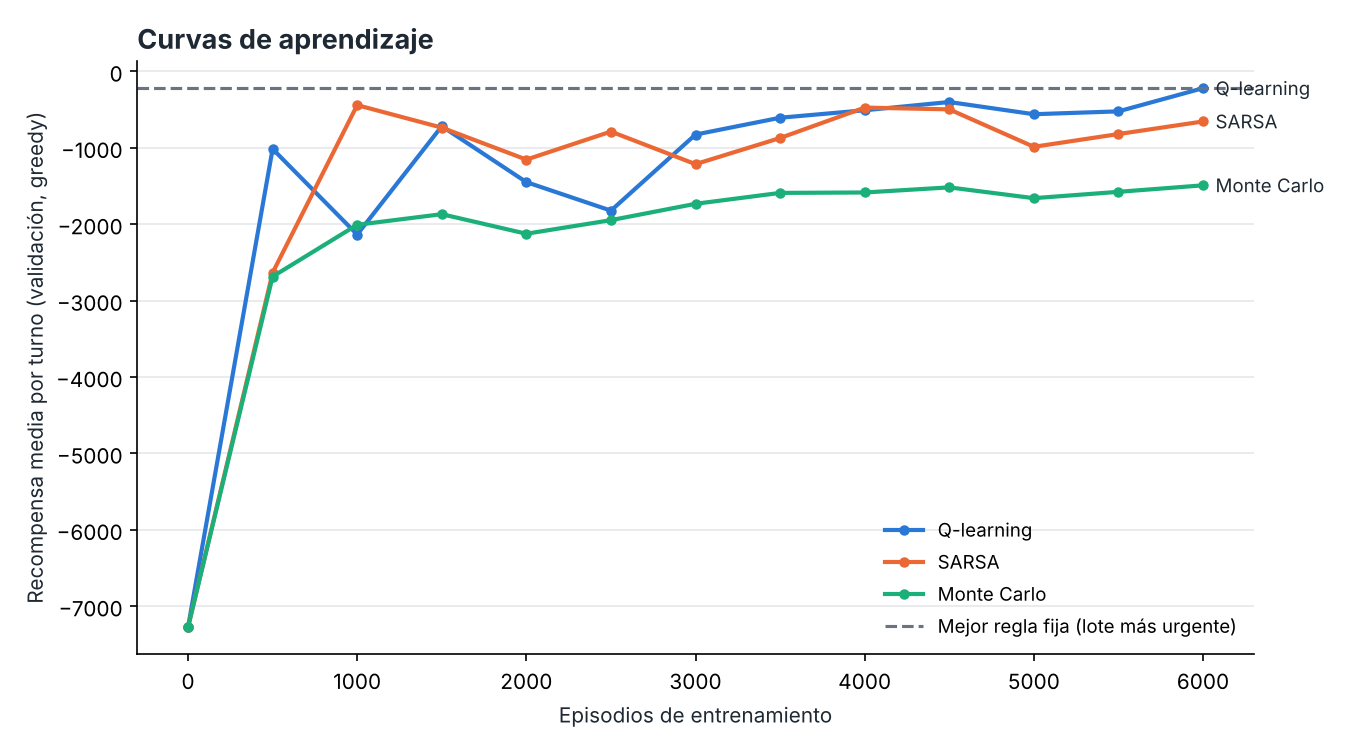
\includegraphics[width=0.82\textwidth]{curvas_aprendizaje.png}
\caption{Curvas de aprendizaje (especificación final, semillas de validación).}
\label{fig:curvas}
\end{figure}

Las oscilaciones, sobre todo las de SARSA, son la huella del aliasing de estados. El estado agregado no
distingue, por ejemplo, una orden recién vencida de una a punto de vencer, ni sabe cuándo se liberará un
operario. Situaciones con consecuencias distintas comparten la misma fila de la Q-tabla, y los valores se
mueven según cuál de ellas haya visto el agente más recientemente. Por eso se guarda la Q-tabla del mejor
punto de control en validación y la evaluación final se hace con semillas distintas.

\subsection{Evaluación en prueba}

El cuadro~\ref{tab:resultados} compara los agentes y las reglas en \TurnosPrueba{} turnos de prueba con las
mismas semillas. La recompensa del agente en prueba (\QLR{}) es peor que la de validación porque la
selección del punto de control tiene un sesgo optimista sobre las semillas de validación; la cifra que vale
es la de prueba.

\begin{table}[H]
\centering\footnotesize
\setlength{\tabcolsep}{4pt}
\begin{tabularx}{\textwidth}{@{}Lrrrrrrr@{}}
\toprule
\textbf{Política} & \textbf{Recompensa} & \textbf{Vencidas} & \textbf{A tiempo} & \textbf{Pend.} & \textbf{Vis./lín.} & \textbf{Viajes} & \textbf{WIP} \\
\midrule
\filas{generado/tabla_resultados.tex}
\bottomrule
\end{tabularx}
\caption{Resultados por turno en \TurnosPrueba{} turnos de prueba ($\pm$: intervalo de confianza del 95\,\% de la media). A tiempo: \% de las órdenes llegadas; Pend.: órdenes pendientes al cierre; Vis./lín.: visitas por línea recogida; WIP: líneas sin asignar en promedio. En promedio llegan \QLLlegadas{} órdenes por turno.}
\label{tab:resultados}
\end{table}

\begin{figure}[H]
\centering
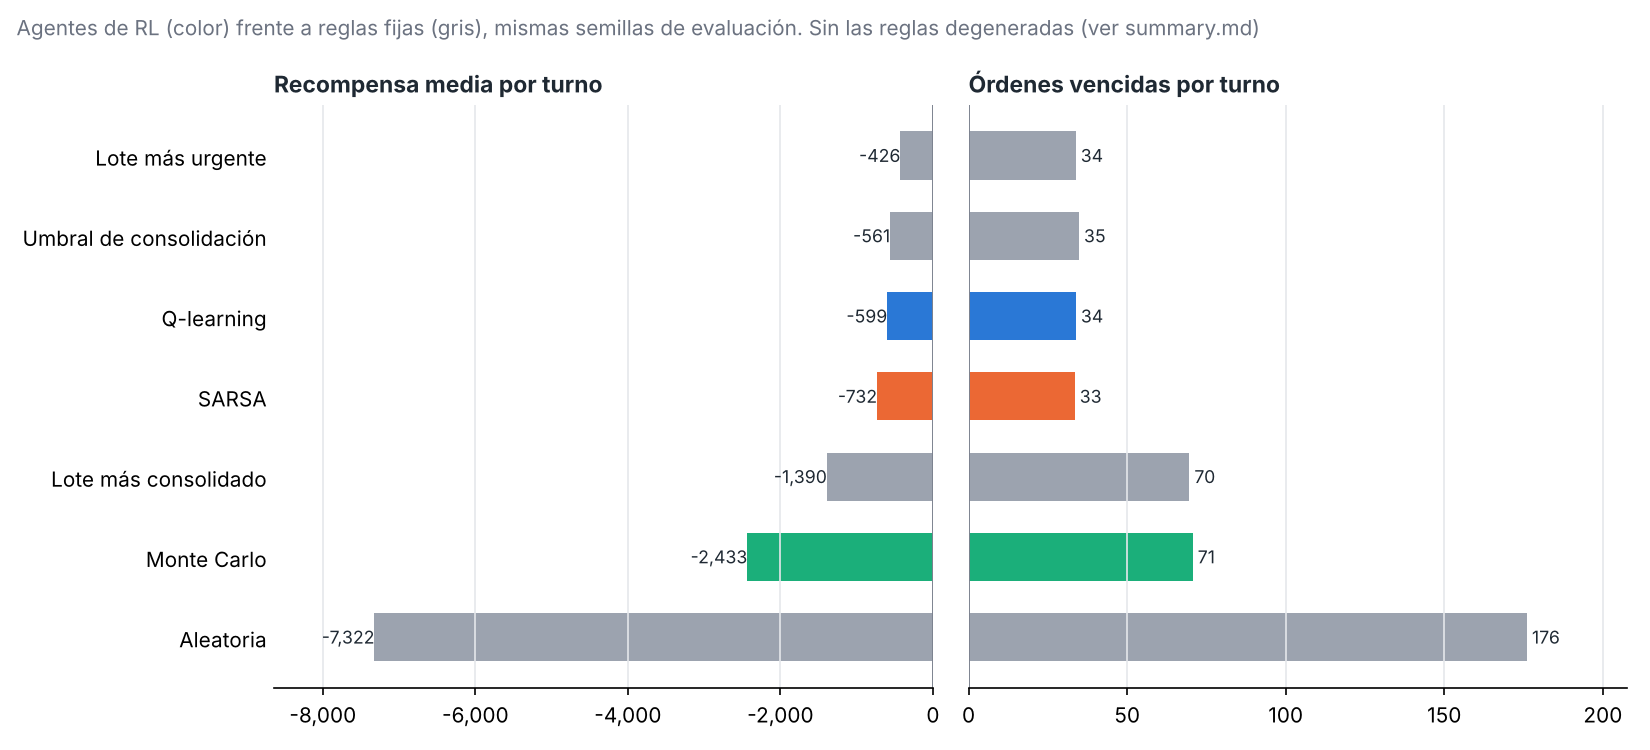
\includegraphics[width=0.92\textwidth]{comparacion.png}
\caption{Recompensa y órdenes vencidas por turno en prueba.}
\end{figure}

Como agentes y reglas se evaluaron sobre los mismos turnos, la comparación más precisa es la diferencia
pareada turno a turno. Frente a la mejor regla, Q-learning tiene:
\begin{itemize}
  \item \textbf{Órdenes vencidas:} \DifQLV{} $\pm$ \DifQLVci{} por turno; no hay diferencia.
  \item \textbf{Viajes:} \DifQLViajes{} $\pm$ \DifQLViajesci{} por turno, unos 11\,\% menos; la diferencia es significativa.
  \item \textbf{Órdenes pendientes al cierre:} \DifQLP{} $\pm$ \DifQLPci{}, ligeramente más.
  \item \textbf{WIP medio:} \DifQLW{} $\pm$ \DifQLWci{} líneas más.
  \item \textbf{Recompensa:} \DifQLR{} $\pm$ \DifQLRci{}; la regla gana.
\end{itemize}
El agente encontró un punto de operación distinto al de la regla: el mismo servicio con menos viajes, a
cambio de más líneas esperando. Con los pesos de la recompensa final ($-0{,}05$ por línea-minuto y $-30$ por
orden pendiente al cierre), ese intercambio resta un poco más de lo que suma. Si en la operación real un
viaje cuesta más que una línea en espera, el punto del agente sería preferible; eso lo decide la operación,
no el algoritmo.

\subsection{Qué aprendió el agente}

El cuadro~\ref{tab:politica} cuenta qué hace la política greedy en cada situación durante \PolTurnos{}
turnos de prueba, frente a la mejor regla. Las columnas corresponden a los comportamientos de la sección
1.1 de la Entrega 1.

\begin{table}[H]
\centering\footnotesize
\setlength{\tabcolsep}{3.5pt}
\begin{tabularx}{\textwidth}{@{}P{2.9cm}P{2.8cm}rRRRRRR@{}}
\toprule
\textbf{Situación} & \textbf{Política} & \textbf{Decis.} & \textbf{Lote zona crítica} & \textbf{Lote otra zona} & \textbf{Lote más consol.} & \textbf{Otro lote} & \textbf{Urgente} & \textbf{Esperar} \\
\midrule
\filas{generado/tabla_politica.tex}
\bottomrule
\end{tabularx}
\caption{Porcentaje de decisiones por situación (solo decisiones con $o\ge1$ y trabajo pendiente).}
\label{tab:politica}
\end{table}

\begin{itemize}
  \item \textbf{D2 (atender lo crítico primero).} Con una orden crítica, el agente despacha la zona crítica en
    el \PolSlotecritica\,\% de los casos. Solo en el \PolSloteotra\,\% atiende otra zona (descuido, N5) y en
    el \PolSesperar\,\% espera.
  \item \textbf{D1 (consolidar).} Cuando alguna zona tiene un SKU pedido por 5 o más órdenes, despacha esa
    zona casi siempre, igual que la regla.
  \item \textbf{D4 (esperar para consolidar).} La diferencia con la regla está en las situaciones sin
    urgencia: el agente espera en el \PolRestoEsperar\,\% de los casos, mientras que la regla nunca espera.
    Ese es el origen de los 10 viajes menos y del WIP adicional. En cambio, en la situación que la Entrega 1
    señalaba como ideal para esperar (alta demanda y consolidación baja) espera solo el
    \PolDcuatroEsperar\,\%: en esos momentos el WIP ya es alto y el costo de esperar también.
\end{itemize}

\subsection{Especificación entregada frente a especificación final}
\label{sec:especificaciones}

Se repitió el entrenamiento completo con la especificación entregada en la Entrega 1
(\code{configs/env\_entrega1.yaml}), sobre la misma demanda y con los mismos hiperparámetros, salvo el
descuento que esa entrega recomendaba ($\gamma=\EGamma$ por decisión). Como las dos recompensas no son
comparables, la figura~\ref{fig:especificaciones} y el cuadro~\ref{tab:especificaciones} comparan
indicadores operativos.

\begin{figure}[H]
\centering
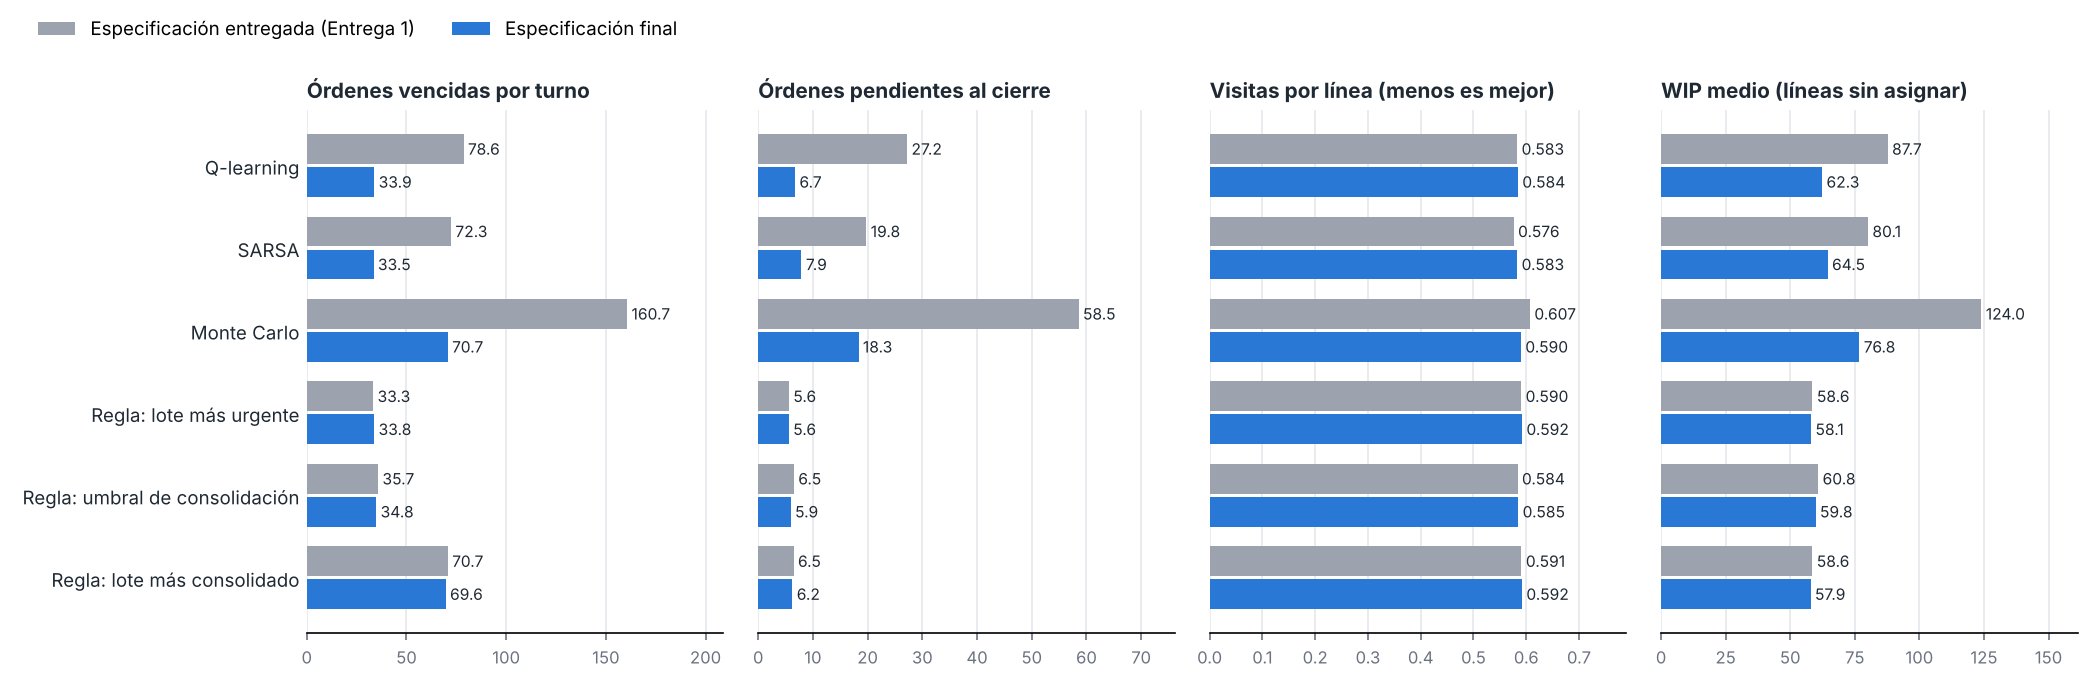
\includegraphics[width=\textwidth]{comparacion_especificaciones.png}
\caption{Indicadores operativos con cada especificación (\TurnosPrueba{} turnos de prueba).}
\label{fig:especificaciones}
\end{figure}

\begin{table}[H]
\centering\footnotesize
\setlength{\tabcolsep}{4pt}
\begin{tabularx}{\textwidth}{@{}Lrrrrrrrr@{}}
\toprule
& \multicolumn{2}{c}{\textbf{Vencidas}} & \multicolumn{2}{c}{\textbf{Pend. cierre}} & \multicolumn{2}{c}{\textbf{Visitas/línea}} & \multicolumn{2}{c}{\textbf{WIP medio}} \\
\cmidrule(lr){2-3}\cmidrule(lr){4-5}\cmidrule(lr){6-7}\cmidrule(lr){8-9}
\textbf{Política} & Entrega 1 & Final & Entrega 1 & Final & Entrega 1 & Final & Entrega 1 & Final \\
\midrule
\filas{generado/tabla_especificaciones.tex}
\bottomrule
\end{tabularx}
\caption{Indicadores por turno con la especificación entregada y con la final.}
\label{tab:especificaciones}
\end{table}

Las reglas fijas obtienen prácticamente los mismos indicadores con las dos especificaciones: la mejor
regla vence \EUrgV{} órdenes con la entregada y \UrgV{} con la final. El simulador y la demanda son los
mismos y saltar el reloj no perjudica a una regla que siempre despacha. Los agentes, en cambio, empeoran
mucho con la especificación entregada: Q-learning vence \EQLV{} órdenes (\DifEQLV{} $\pm$ \DifEQLVci{} más
que la regla) y deja \EQLP{} pendientes al cierre. La diferencia está en lo que la recompensa entregada
le enseña al agente, no en el problema.

El mecanismo se ve en la política aprendida: con una orden crítica pendiente, el agente entrenado con la
especificación entregada espera en el \PolESesperar\,\% de los casos, contra el \PolSesperar\,\% del agente
final. Con el reloj saltando hasta que un operario quede libre, la acción que asigna al último operario
libre se lleva sin descuento todos los vencimientos del salto, a veces más de 20 minutos. Esperar, en
cambio, reparte esos costos en pasos de 2 minutos descontados. El agente aprende que despachar sale caro,
lo contrario de lo que se quería. Los cambios del cuadro~\ref{tab:cambios} corrigen ese sesgo y los
incentivos que premiaban fragmentar lotes y esperar por esperar. Una limitación de esta comparación es que
evalúa los cambios en conjunto, no cada uno por separado.

\subsection{Limitaciones}

\begin{itemize}
  \item \textbf{Aliasing de estados.} La observación agregada omite la identidad y la antigüedad de las
    órdenes, los trabajos en ejecución y la hora del turno, así que el problema no es estrictamente de Markov.
    Es la principal razón de las oscilaciones y de que el agente no supere a la mejor regla.
  \item \textbf{Escala.} Se usó la versión de 2 zonas (9\,409 estados; el agente visitó \QLEstados{}). La de
    4 zonas tiene 7,4 millones de estados y requeriría aproximación de funciones en lugar de una tabla.
  \item \textbf{Simulador.} Los resultados dependen de supuestos de demanda y tiempos que no se calibraron
    con datos reales.
\end{itemize}

Como trabajo futuro, agregar la franja del turno y la antigüedad del WIP al estado reduciría el aliasing.
También convendría calibrar el peso del WIP frente al costo de un viaje con datos de la operación.


% =====================================================================
\section{Entregables y reproducción}

\begin{table}[H]
\centering\small
\begin{tabularx}{\textwidth}{@{}P{6.4cm}L@{}}
\toprule
\textbf{Archivo} & \textbf{Contenido} \\
\midrule
\code{results/models/q\_learning.npz} & Q-tabla del agente entregado (se carga con \code{TabularAgent.load}) \\
\code{results/models/*\_qtable.csv} & Q-tablas legibles de los tres algoritmos \\
\code{results/figures/demo.mp4} & Video de un turno completo del agente \\
\code{results/logs/} & Registros de entrenamiento, curvas, evaluación por turno y resúmenes \\
\code{results/entrega1/} & Lo mismo con la especificación entregada \\
\code{src/}, \code{experiments/}, \code{tests/} & Código completo y 29 pruebas automáticas \\
\bottomrule
\end{tabularx}
\caption{Entregables en el repositorio \href{https://github.com/panamiguell/rl-warehouse-agent}{panamiguell/rl-warehouse-agent}.}
\end{table}

{\small
\begin{verbatim}
conda env create -f environment.yml && conda activate rl-warehouse-agent
python -m pytest                                    # 29 pruebas
python experiments/train.py                         # final, unos 40 min
python experiments/train.py --config configs/env_entrega1.yaml --out results/entrega1
python experiments/compare_specs.py
python experiments/demo.py --model results/models/q_learning.npz
\end{verbatim}
}

Todos los resultados son reproducibles con las semillas fijas del código.

\end{document}
